% \setchapterpreamble[u]{\margintoc}
\chapter{Introduction}
\labch{intro}

Type theory is set at the interface between programming and formal logic,
feeding off and nourishing both worlds. Proof assistants can be built on it,
making them full-fledged programming languages as well, with the added benefit
of producing certified programs.

My main interest lies in the study of type theory while relying on the tools it
provides: I study type theory \emph{within} type theory.
As such I focused on the formalisation of type theory in the \Coq proof
assistant~\sidecite[-0.7cm]{coq} and particularly on two points:
\marginnote[0.7cm]{
  Reflection is defined in \arefsubsec{ett-def}, and weak equality in
  \arefsubsec{wtt}, both in \refch{flavours}.
}
\begin{itemize}
  \item How can we effectively turn a proof using a very strong notion of
  equality called \emph{reflection}, into a proof relying on a very weak notion
  of equality?
  \item How can we improve the trust in our system, in my case \Coq, using this
  system itself as a framework to study it?
\end{itemize}

\paradot{Contributions}
My contributions will mainly be found in \avrefpart{elim-reflection}, and
\avrefpart{coq-in-coq}, corresponding to the following published
articles~\sidecite{winterhalter:hal-01849166,sozeau2019coq,sozeau:hal-02167423}.
While the chapters before these two parts are mainly introductory and
corresponding to a rough state-of-the-art, they actually contain other
contributions, namely work I did with Andrej Bauer on the cardinal model
in \nrefch{models} that we did not publish, and work I did with Andrej Bauer
and Philipp Haselwarter on formalising type theory called
\ftt~\sidecite{formaltypetheory} and that I present briefly in
\nrefch{formalisation}.

\section{Proof assistants}

One of my goals is improving and understanding better proof assistants, but what
is a proof assistant?
I think we can see them as chatbots---that is, those programs that you can
converse with---that are there to help you assert and prove theorems.
They are not particularly smart and will not get the job done for you, but they
are very annoying because they do not always understand what you say and you
have to be very precise or they will point out your mistakes.

\marginnote[1.2cm]{
  The user will have blue speech bubbles, slightly on the left, while the proof
  assistant will answer in green (for good) or red (for bad) on the right-hand
  side.
}%
\begin{center}
  
\includegraphics[width=0.6\textwidth]{coq-chatbot.pdf}
\end{center}

Here, I represent the user on the left, conversing with the proof assistant, on
the right, that I picture as a laptop with a rooster inside.

Let us now see in detail how such a conversation can go.

\begin{center}
  
\includegraphics[width=0.8\textwidth]{modern-art.pdf}
\end{center}

\marginnote[0.1cm]{
  When I say they agree, I mean that, in particular, the proof assistant has
  basic knowledge of cats and boxes, for instance you don't need to show it
  that a cat is a feline.
  It also knows what each box contains, for instance that the fourth box
  contains a red cat.
}
This piece of modern art will be the setting for the exchange between the user
and the proof assistant, and we will assume they both agree on it.
We have cats in boxes (although one of the cats is rather a lion), of different
colours, and subject to different gravitation forces.

At the beginning, the user makes their purpose know to the proof assistant,
saying for which theorem they require their assistance.

\begin{center}
  
\includegraphics[width=0.8\textwidth]{iwanterror.pdf}
\end{center}

The sentence above doesn't sound like a statement we can prove, and the proof
assistant will rightfully complain.

\begin{center}
  
\includegraphics[width=0.8\textwidth]{error-incomplete.pdf}
\end{center}

Indeed, we were to fast and forgot half of what we wanted to say. Next we give
it a complete sentence.

\begin{center}
  
\includegraphics[width=0.8\textwidth]{iwant-is.pdf}
\end{center}

This time, the statement is slightly incorrect, or not precise enough for our
good assistant.

\begin{center}
  
\includegraphics[width=0.8\textwidth]{error-box-feline.pdf}
\end{center}

We have to revise our wanted theorem, and realise that we do not want to prove
that all boxes are feline, although a human might understand what we mean by
that, but that all of the boxes contain, each, a feline.

\begin{center}
  
\includegraphics[width=0.8\textwidth]{box-contains-feline.pdf}
  
\includegraphics[width=0.8\textwidth]{how-to-prove.pdf}
\end{center}

The proof assistant has now understood what we meant. The interactive part of
the prove now begins. We want to prove a property on the boxes, as there are
four to consider, we can tell the proof assistant that we intend to look at each
case, one by one.

\begin{center}
  
\includegraphics[width=0.8\textwidth]{convo7.pdf}
  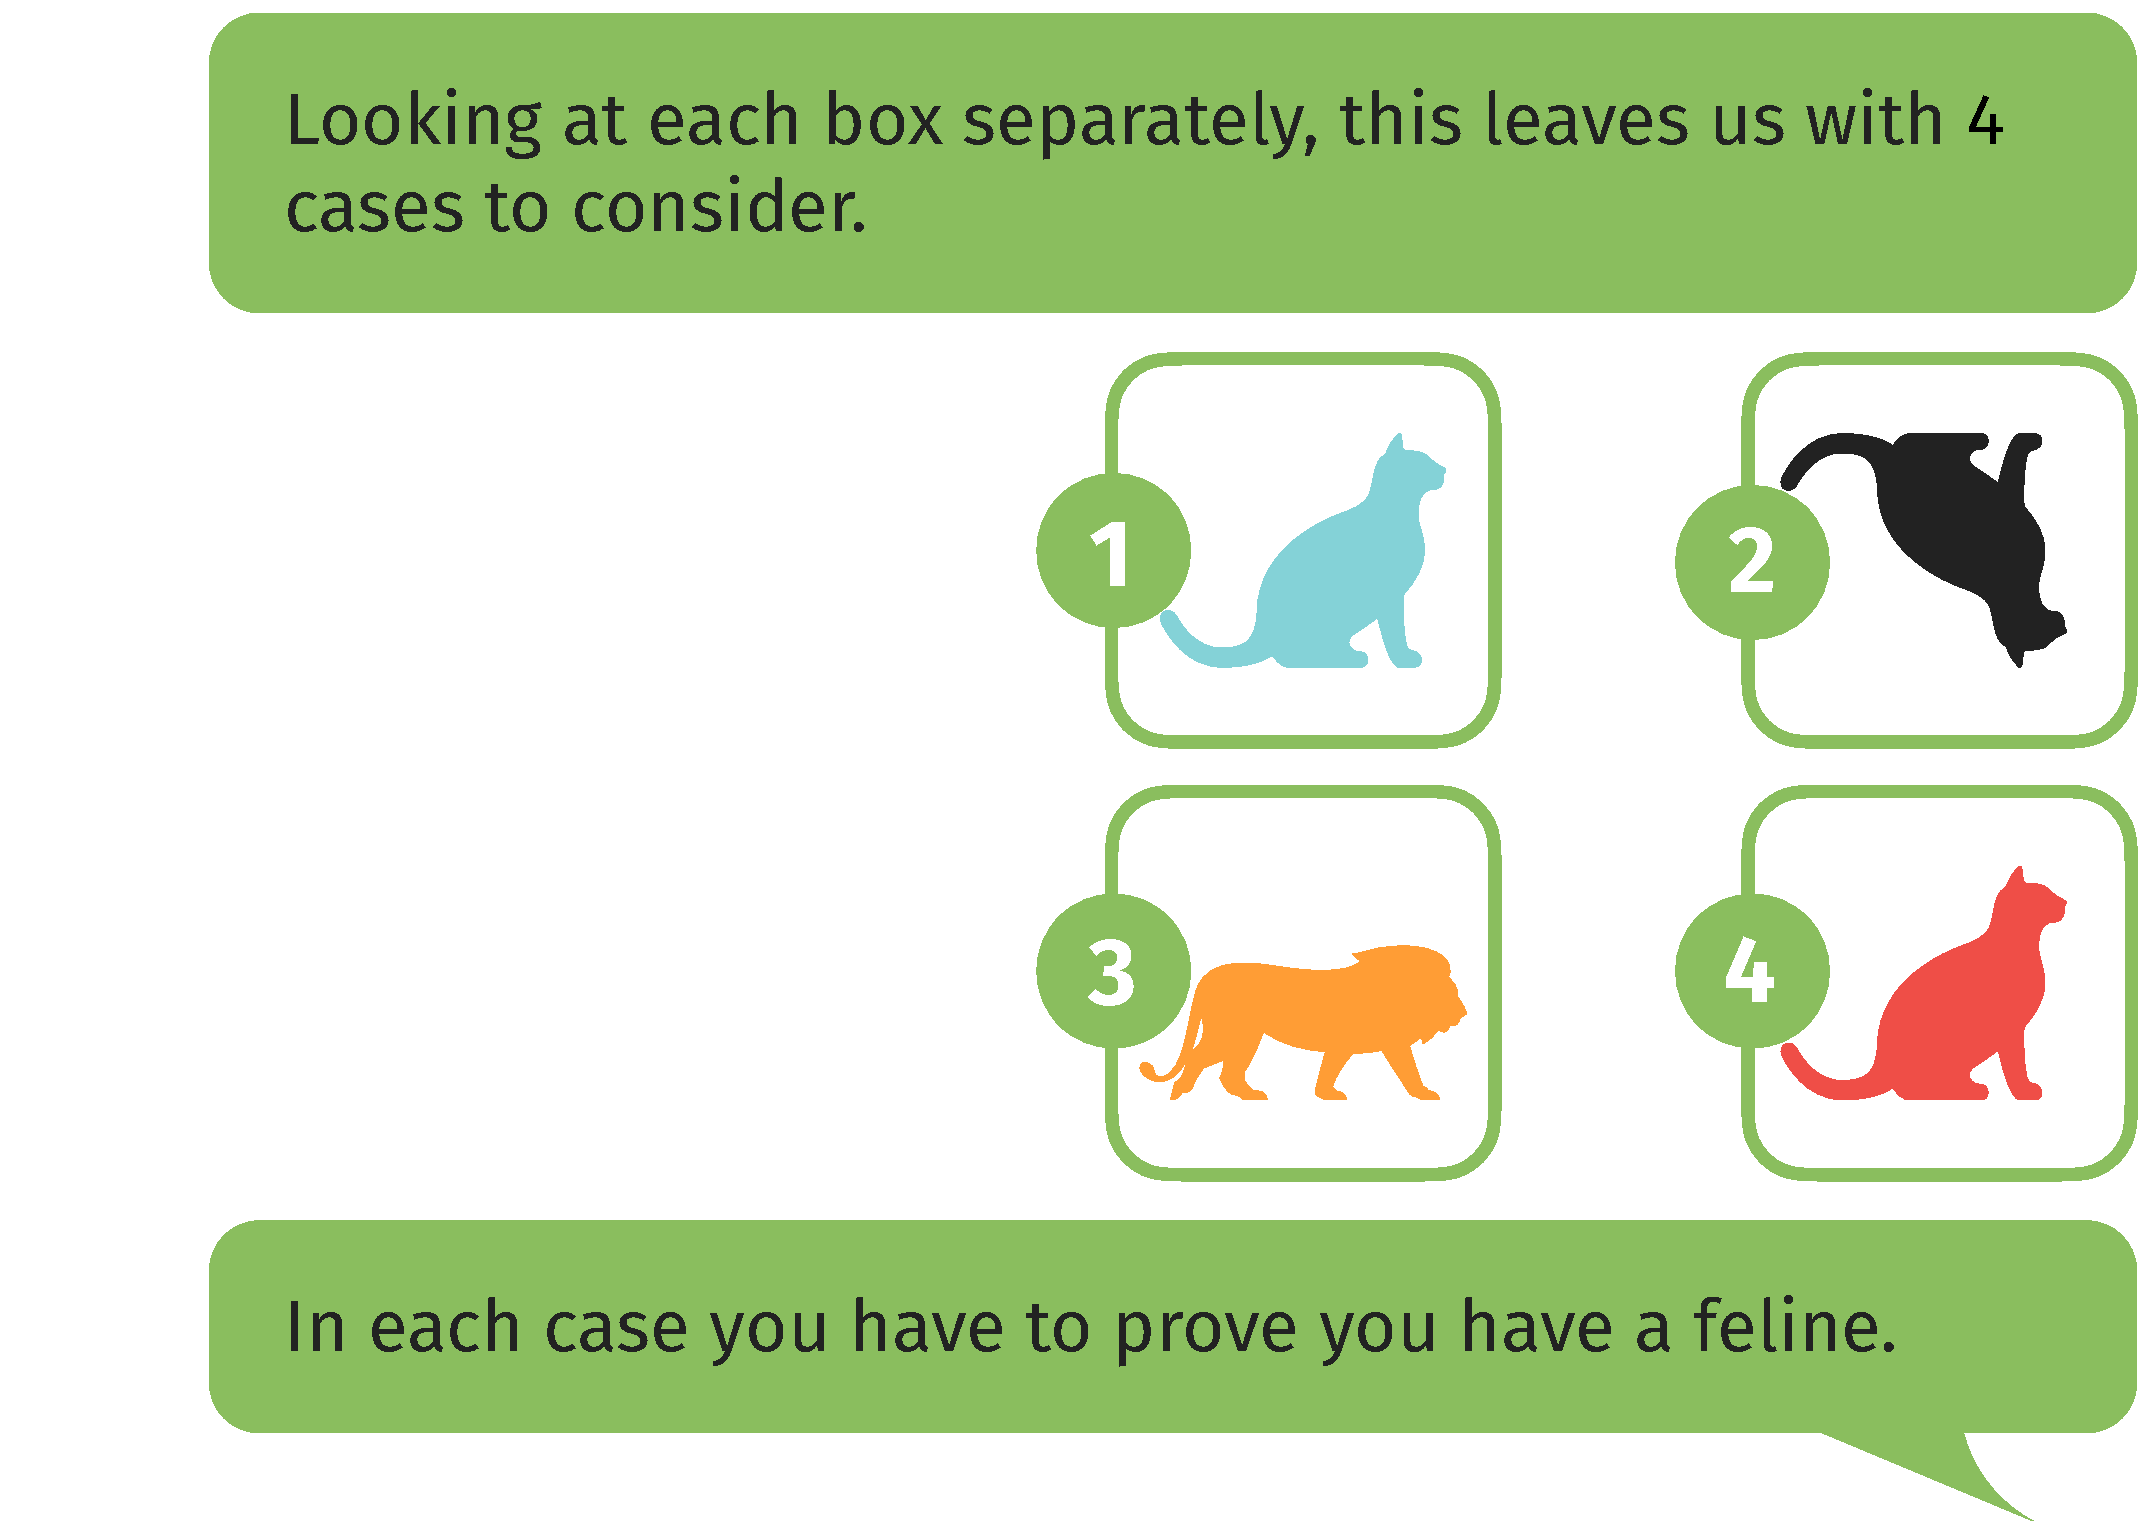
\includegraphics[width=0.8\textwidth]{convo8.pdf}
\end{center}

We are presented with four cases, and as many statements to prove.
In this case, we are rather lazy, especially since all four cases will be
similar. Fortunately for us, the proof assistant is capable of understanding
that you want to deal with several cases in similar ways, \emph{and} is also
capable of doing very basic proofs without the user.

\begin{center}
  
\includegraphics[width=0.8\textwidth]{convo9.pdf}
  
\includegraphics[width=0.8\textwidth]{convo10.pdf}
\end{center}

Once the proof is complete, the proof assistant tells you so and you can move on
to other theorems to prove. I already showed that you have to be explicit and
non ambiguous when talking to the proof assistant. You also have to be correct.
The proof assistant will not trust blindly into what you say.
%
Let us now consider a theorem that is not provable.

\begin{center}
  
\includegraphics[width=0.8\textwidth]{convo11.pdf}
  
\includegraphics[width=0.8\textwidth]{how-to-prove.pdf}
  
\includegraphics[width=0.8\textwidth]{convo7.pdf}
  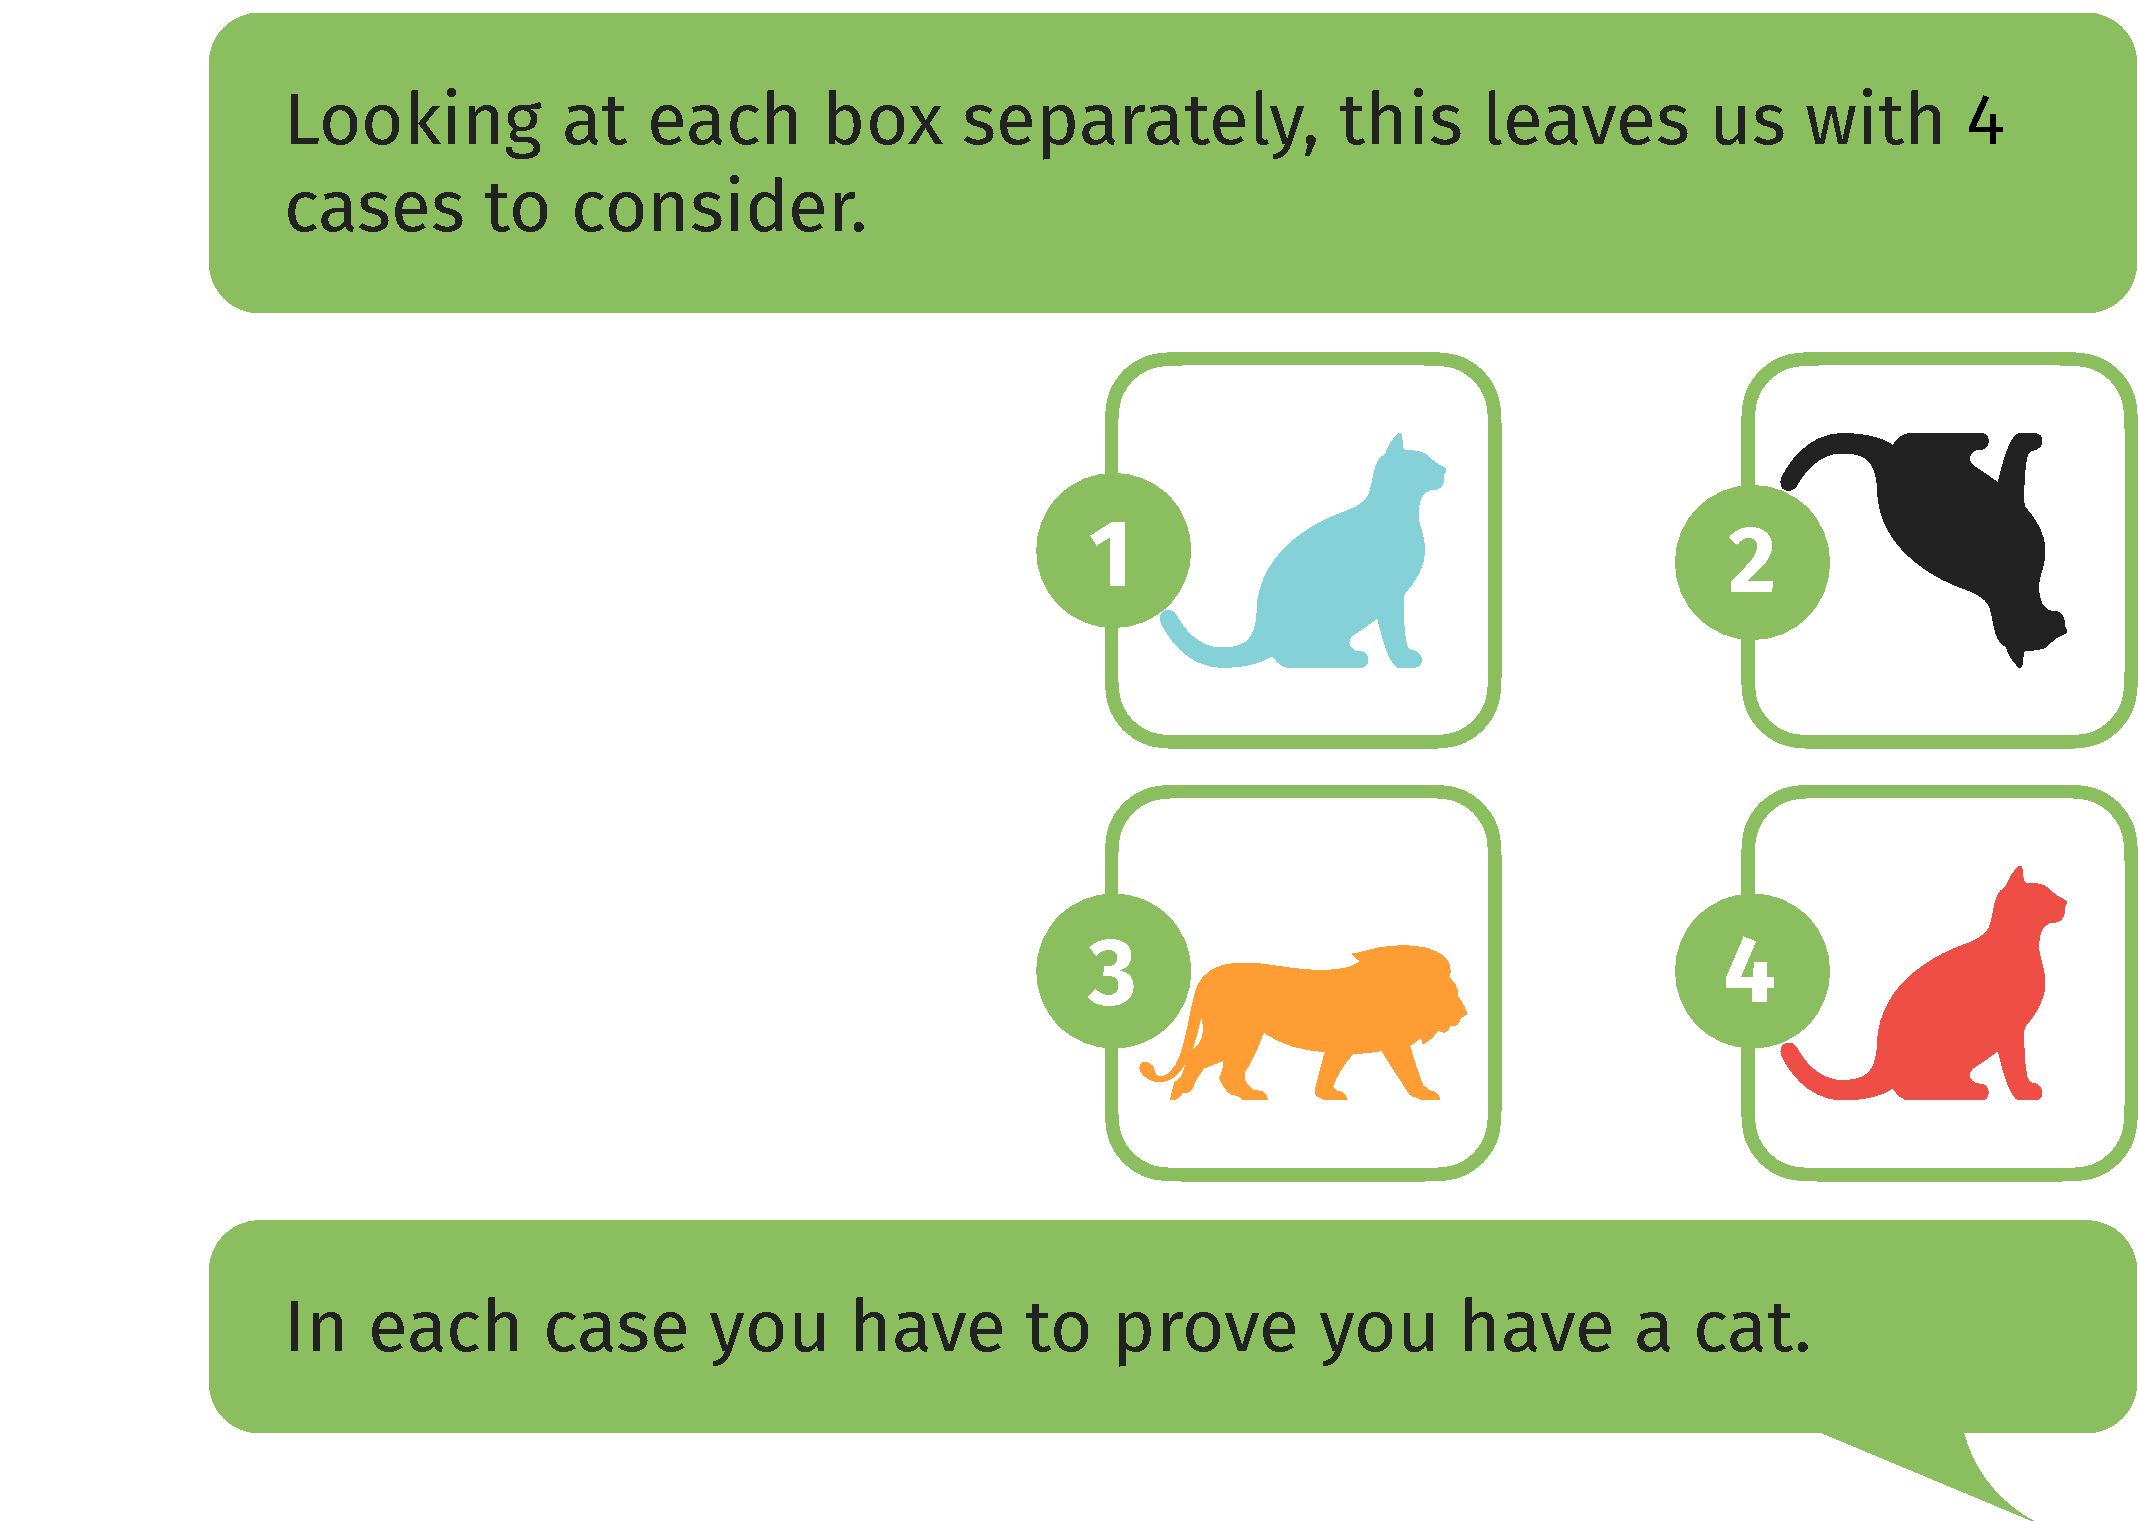
\includegraphics[width=0.8\textwidth]{convo12.pdf}
  
\includegraphics[width=0.8\textwidth]{convo9.pdf}
  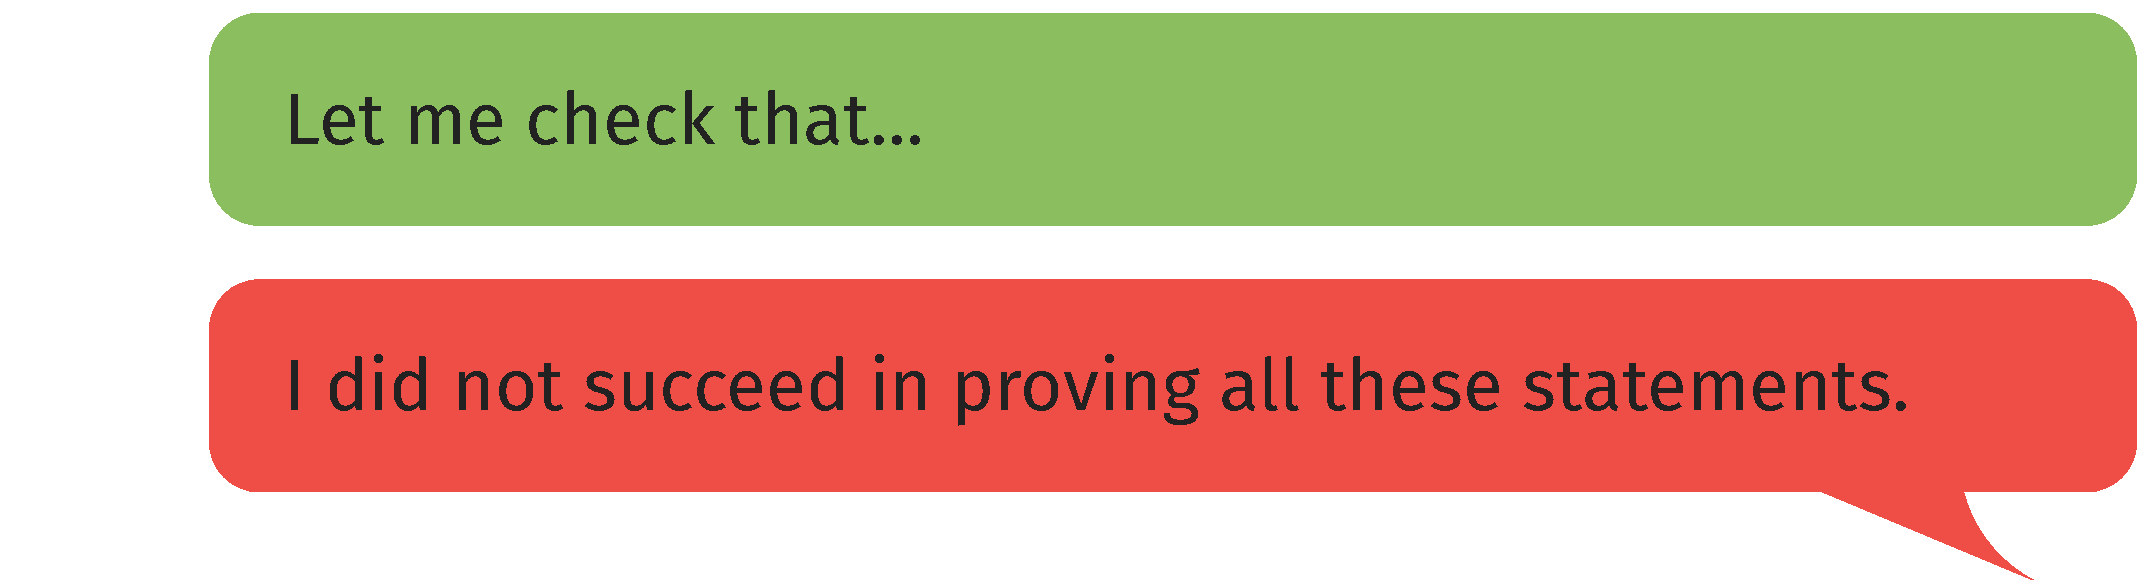
\includegraphics[width=0.8\textwidth]{convo13.pdf}
\end{center}

Here the proof assistant tells us that not all cases are trivial so we decide
to go over them one by one to understand what is wrong.

\begin{center}
  
\includegraphics[width=0.8\textwidth]{convo-focus.pdf}
  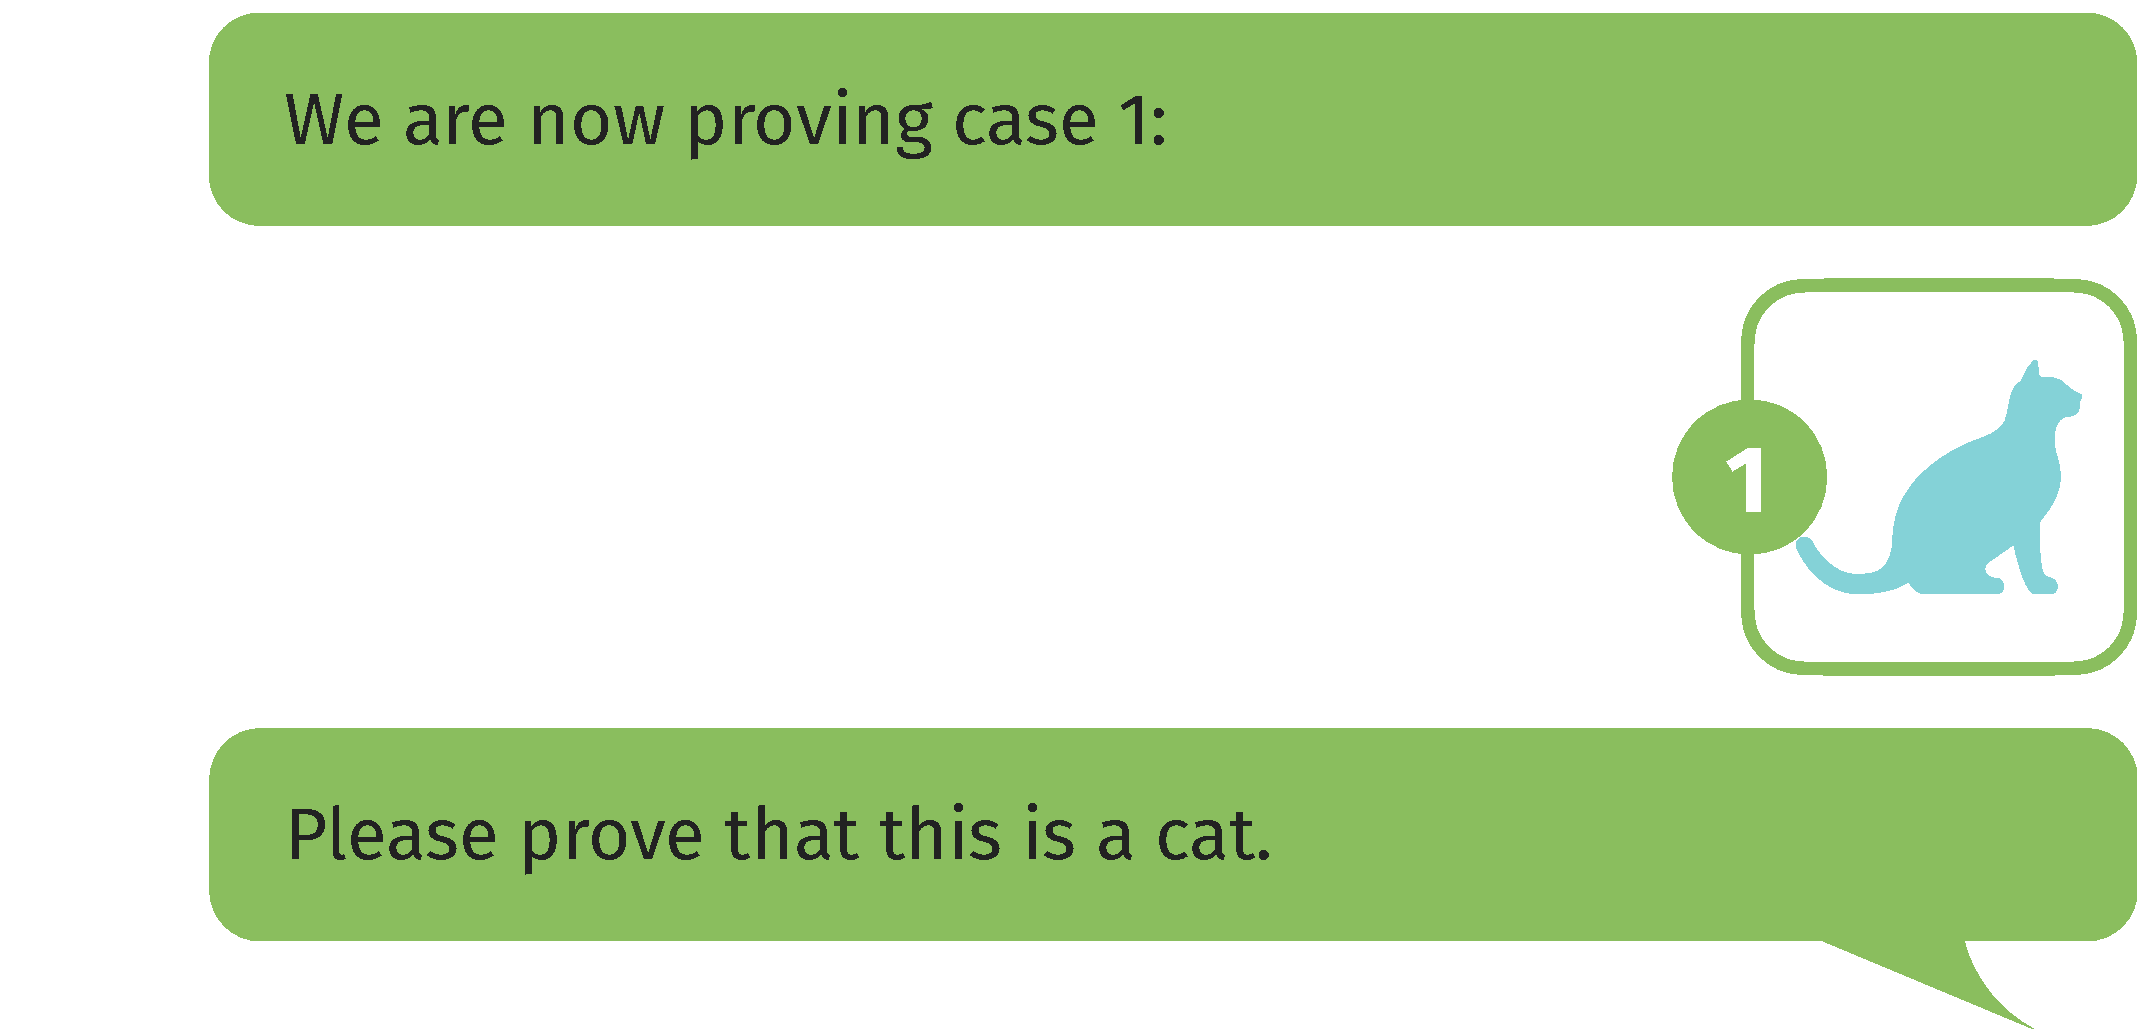
\includegraphics[width=0.8\textwidth]{convo-case1.pdf}
\end{center}

When we focus on a case, the proof assistant reminds us of what we have to prove
specifically. Here we revert to using our earlier strategy and simply say that
it is plain to see.

\begin{center}
  
\includegraphics[width=0.8\textwidth]{convo-trivial.pdf}
  
\includegraphics[width=0.8\textwidth]{convo-indeed.pdf}
  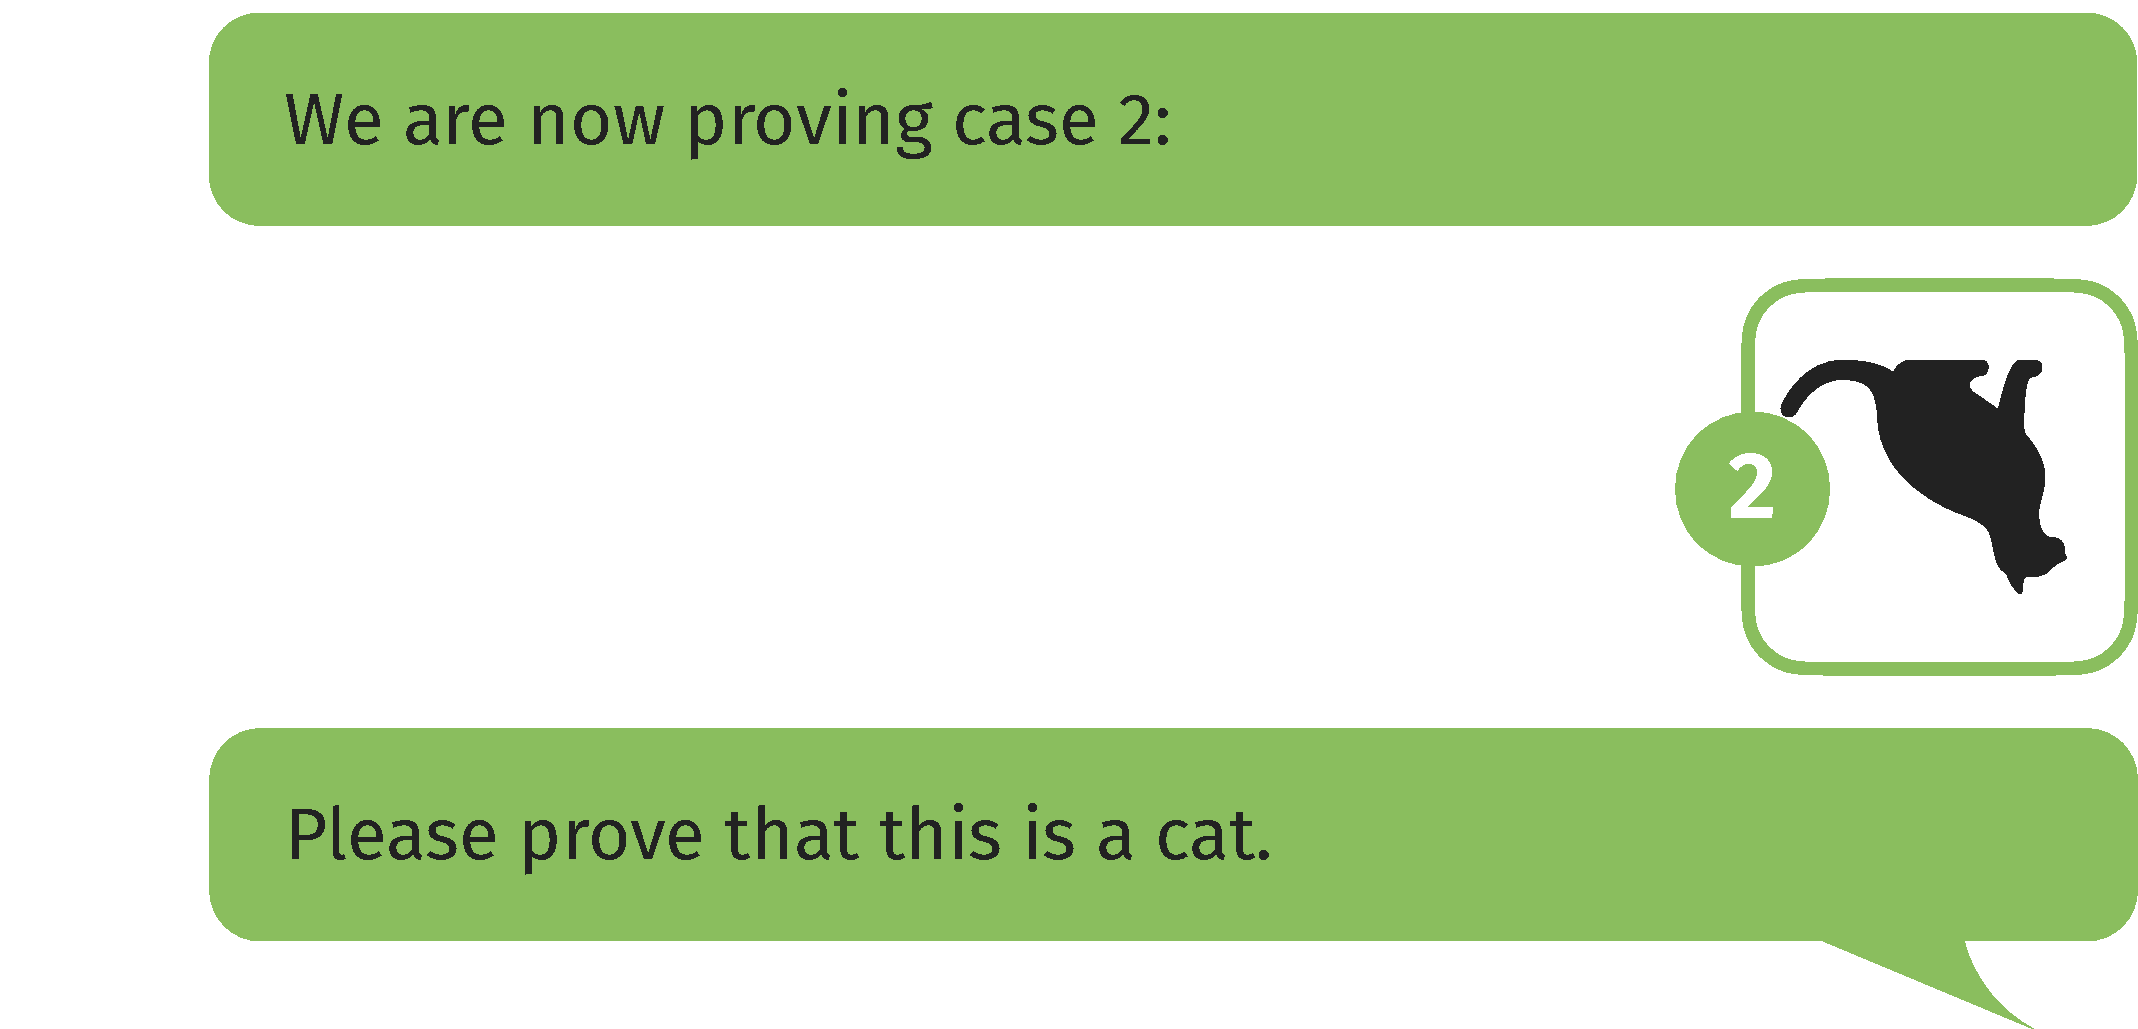
\includegraphics[width=0.8\textwidth]{convo-case2.pdf}
  
\includegraphics[width=0.8\textwidth]{convo-trivial.pdf}
  
\includegraphics[width=0.8\textwidth]{convo-indeed.pdf}
  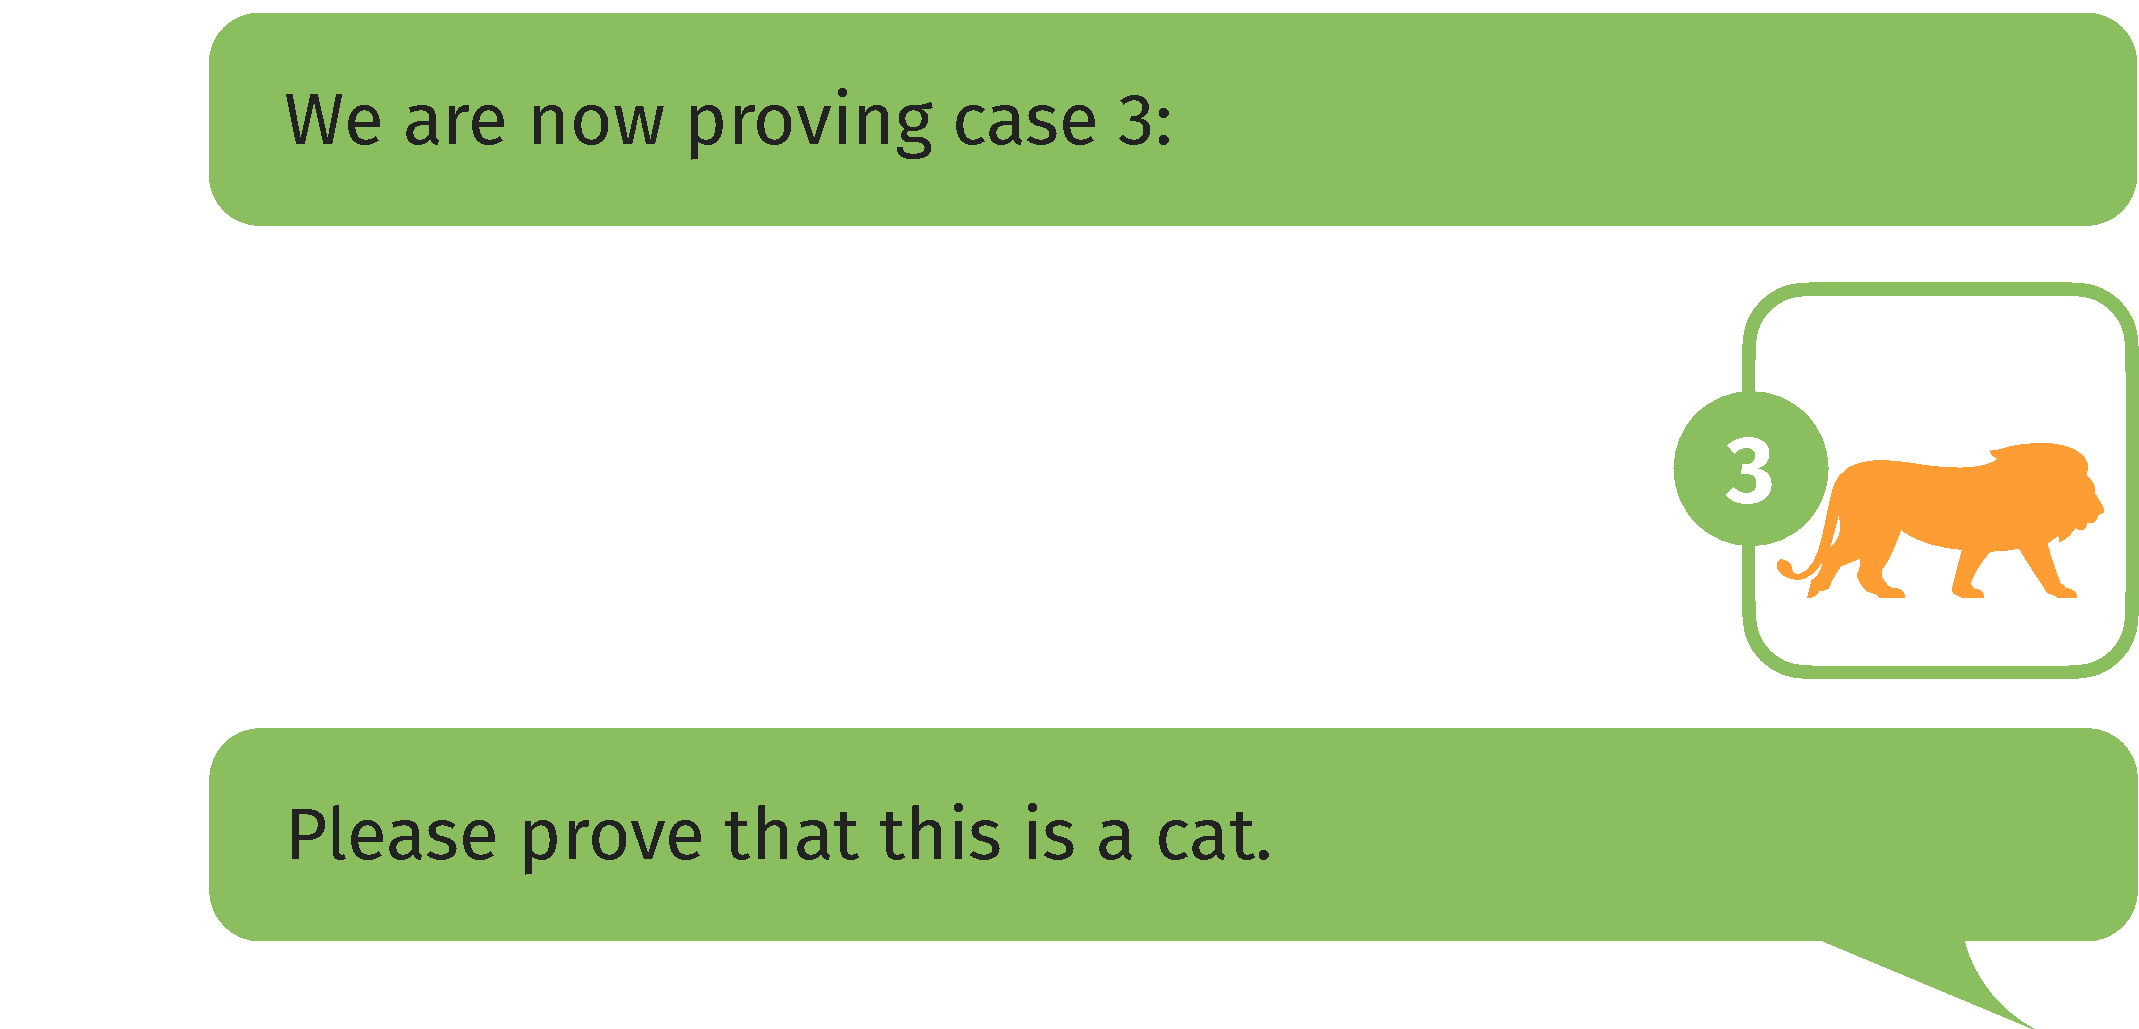
\includegraphics[width=0.8\textwidth]{convo-case3.pdf}
  
\includegraphics[width=0.8\textwidth]{convo-abort.pdf}
\end{center}

This time, we see we do not have a cat so we do not even try to prove it.
We abort the proof, that is we give up on proving a statement we know to be
wrong now.
One important thing to note here is that the proof assistant still does not
know the statement is incorrect, only that the proof attempt was itself invalid.
We can show it to be incorrect by proving the converse:

\begin{center}
  
\includegraphics[width=0.8\textwidth]{conv-exists.pdf}
  
\includegraphics[width=0.8\textwidth]{how-to-prove.pdf}
\end{center}

The easiest way of proving that something exists is by providing a so-called
\emph{witness} of existence. Here we are looking for a box which does not
contain a cat, there is only one box with no cat in it, as we found out during
our previous proof, the third.

\begin{center}
  
\includegraphics[width=0.8\textwidth]{convo-take-third.pdf}
  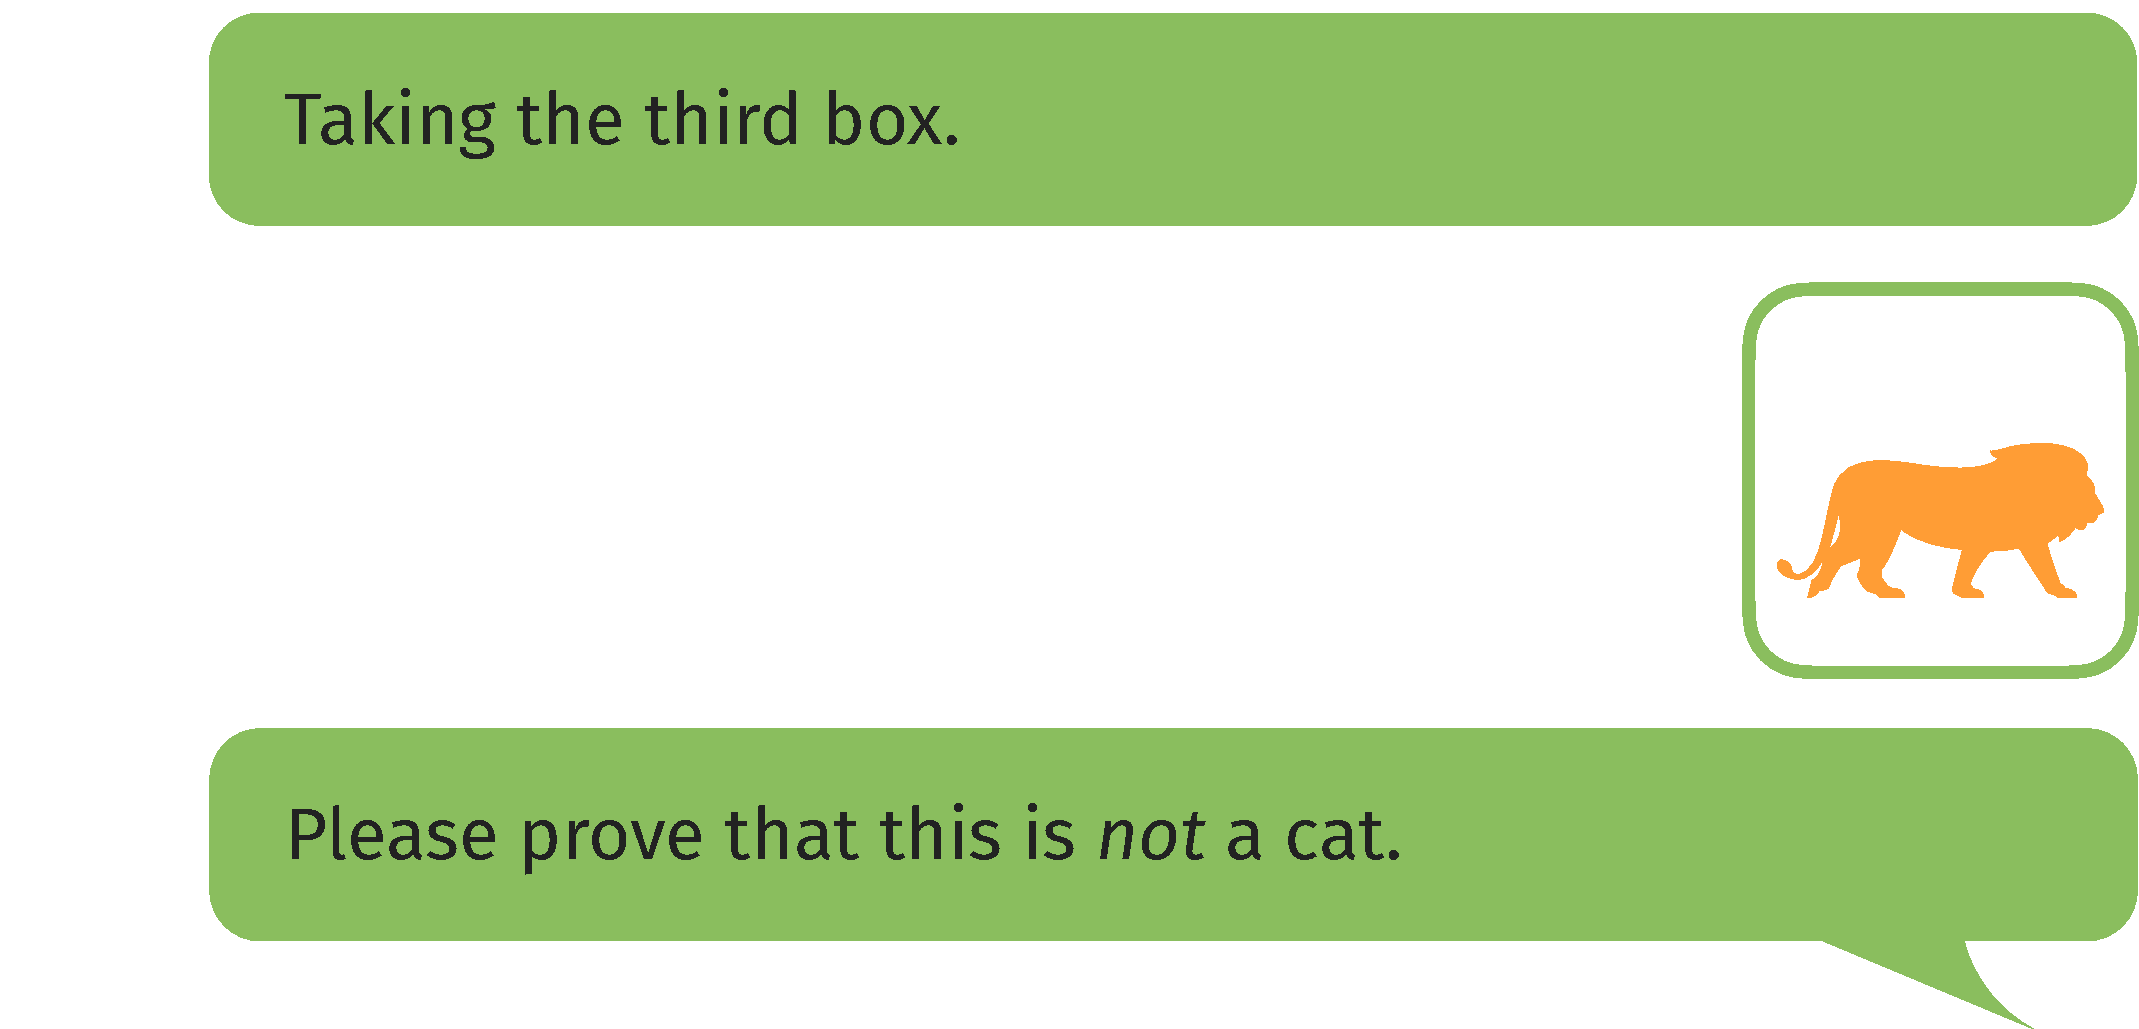
\includegraphics[width=0.8\textwidth]{convo-after-exists.pdf}
  
\includegraphics[width=0.8\textwidth]{convo-trivial.pdf}
  
\includegraphics[width=0.8\textwidth]{convo-indeed.pdf}
  
\includegraphics[width=0.8\textwidth]{convo-proven.pdf}
\end{center}

A proof assistant is thus both helping us do proofs by building parts of it on
its own, and verifying that they are correct, for instance by not forgetting one
case where we had a lion rather than a cat.

Proof assistants are also interesting and useful for other people than the user
doing the proof. Say that I have proven a complicated theorem using my favourite
proof assistant, people who trust my proof assistant will simply have to ask it
if it agrees with my claim.
In fact, proof assistants usually generate so-called \emph{certificates} that
can be checked by others without having to understand the details of the proof.
\marginnote[1.6cm]{
  The picture can be misleading, I am really talking about a concrete object
  that people can run through their own proof assistant to check that a proof
  is indeed valid.
}
\begin{center}
  
\includegraphics[width=0.5\textwidth]{cerificate.pdf}
\end{center}

Even then, why should we trust the proof assistant? What exactly can we prove
with them? And how can we make them better?
Part of my work is focused on these questions, and on the study of proof
assistants based on something called type theory.

\section{Proofs, types and programs}

In order to explain the title ``Formalisation and Meta-Theory of Type Theory''
I need to explain what \emph{type theory} is. Even before that, I believe I have
to introduce \emph{proof theory} (\refch{proof-theory}): the study of proofs
themselves. Indeed, in order to build a proof assistant one needs to understand
what a proof is, formally, \ie in very precise and non-ambiguous terms.

It turns out that certain formal notion of proofs have intricate relations with
programming as we shall see in \refch{simple-types}. The idea is that programs
can be seen as proofs, and proofs as programs.
For instance a proof that a proposition \(A\) implies the proposition \(B\)
is a program that takes a proof of \(A\) as input and outputs a proof of \(B\).
Such a program is given type \(A \to B\). Types are a way of describing the data
return by a program. Student will often write the infamous leap year function
which, given a year as an integer (described by the type
\mintinline{ocaml}{int}), returns whether it is a leap year or not. This binary
information---yes or no---is encoded into what we call booleans
(\mintinline{ocaml}{bool}).
The Curry-Howard correspondence states that programs of type \(A\) can be seen
as proofs of propositon \(A\) and vise-versa.

In \refch{dependent-types}, I finally describe what I call type theory.
Type theory is framework taking advantage of this correspondence and is thus at
the core of well-known proof assistants such as \Coq~\sidecite[-0.85cm]{coq} and
\Agda~\sidecite[0.25cm]{norell2007towards}. I myself am a \Coq user and this
thesis is written with a focus on this proof assistant and its foundations.
In \refch{usual-defs}, I describe usual definitions that come with type theory.
I explain how we can reason in such a setting with more than implications.
\sidedef[-1cm]{Induction on natural numbers}{%
  If \(P(n)\) is a property on natural number \(n\), then if we have
  \begin{enumerate}
    \item \(P(0)\);
    \item \(P(m)\) implies \(P(m+1)\) for any \(m\);
  \end{enumerate}
  then we have \(P(n)\) for any \(n\).
}%
This is where I introduce for instance the way of doing induction on natural
numbers in type theory.

\refch{flavours} is dedicated to different formulations and variants of type
theory. Indeed, there is not just one such theory. Different type theories have
different properties, I catalogue the most important ones while telling which
theory enjoys which in a summarising table.

The remaining of the introductory part will focus more on the `meta-theory'
part of the title. While the theory is where you conduct your proofs and write
your programs, the meta-theory is where you reason about the theory itself!
In \refch{models}, I explain how we can build so-called models of type theory,
which consist in interpreting the theory and giving it meaning---or
\emph{semantics}---inside the meta-theory. At the end, I hint at how the
meta-theory can even be a form of type theory itself. The representation of
type theory inside itself is the subject of \refch{formalisation} while
\refch{translations} focuses on how we can give meaning to a type theory, using
another type theory.

\section{Elimination of reflection}

Next, we have \arefpart{elim-reflection}. The title can be scary but it falls in
the category of ``what can I prove with my proof assistant?'' and
``how can I improve proof assistants?''

Type theory is at the interface of logic and programming. Traditionally,
programming languages are designed with the idea that, eventually, programs
will be \emph{run}, or \emph{evaluated}. In other programs \emph{compute}.
Now, computation is also an important part of type theory. Computation
corresponds to the simplification of proofs, but also more importantly it
embodies the notion of \emph{constructivism}. Say, in the example of earlier,
that you prove that ``there exists a cat with a gravity issue,'' if you execute
this proof, it will compute and yield two important informations: who is the
guilty cat---in this case the black one in the second box---and why it has
gravity issues (as another proof).

Computation is also useful when doing proofs. For instance, \(2 + 2\) \emph{is}
\(4\), so no need to carry around any informaiton relating the two. \(2 + 2\)
will evaluate to \(4\), so two sets of two catboxes is really just a set of four
catboxes.

Now there are various degrees of computation that can be put inside a type
theory, and one might wonder what impacts it has on it. I present a spectrum
of three different theories. On one side a theory, called \acrfull{ETT},
which is very liberal with respect to computation in that it identifies any two
things that we prove or assume equal, in such a setting, computation is no
longer directed and we simply talk about things being \emph{equal}.
This principle, turning a proof into an equality, is called \emph{reflection} of
equality.
The other extreme is a theory, called \acrfull{WTT}, where we remove the very
notion of computation. In the middle, we have \acrfull{ITT} which has a
`regular' notion of computation, defined as the evaluation of functions. The
latter is the base for \Coq and \Agda.

My contribution is a translation from \acrshort{ETT} to \acrshort{ITT} and
\acrshort{WTT}, showing that computation is not an essential property---albeit
highly practical---of type theory. The translation is done in type theory
itself---in this case \Coq---and as such provides a program turning a proof in
\acrshort{ETT} into a proof in \acrshort{ITT} or \acrshort{WTT} that can
actually be used to compute new proofs.

\section{A verified type-checker for \Coq, in \Coq}

Finally, in \arefpart{coq-in-coq}, I will address the question ``How can we
increase the trust in a proof assistant?'' Focusing once more on \Coq, I present
a verification of \Coq's kernel, using \Coq itself.

\Coq features a kernel that is a rather small program that checks that proofs
are indeed correct. The interactive part of the proof assistant, as well as the
automation---\ie the thing that makes the proof assistant find proofs for
us---are not part of the kernel and rather built above it.
If you want, the part that checks the certificates is separate from the rest
and as such is easier to survey.

\marginnote[1.2cm]{
  The egg on the right represents the kernel. The proof assistant essentially
  sends it the certificate it generated after discussing with the user and the
  kernel validates it (or not).
}
\begin{center}
  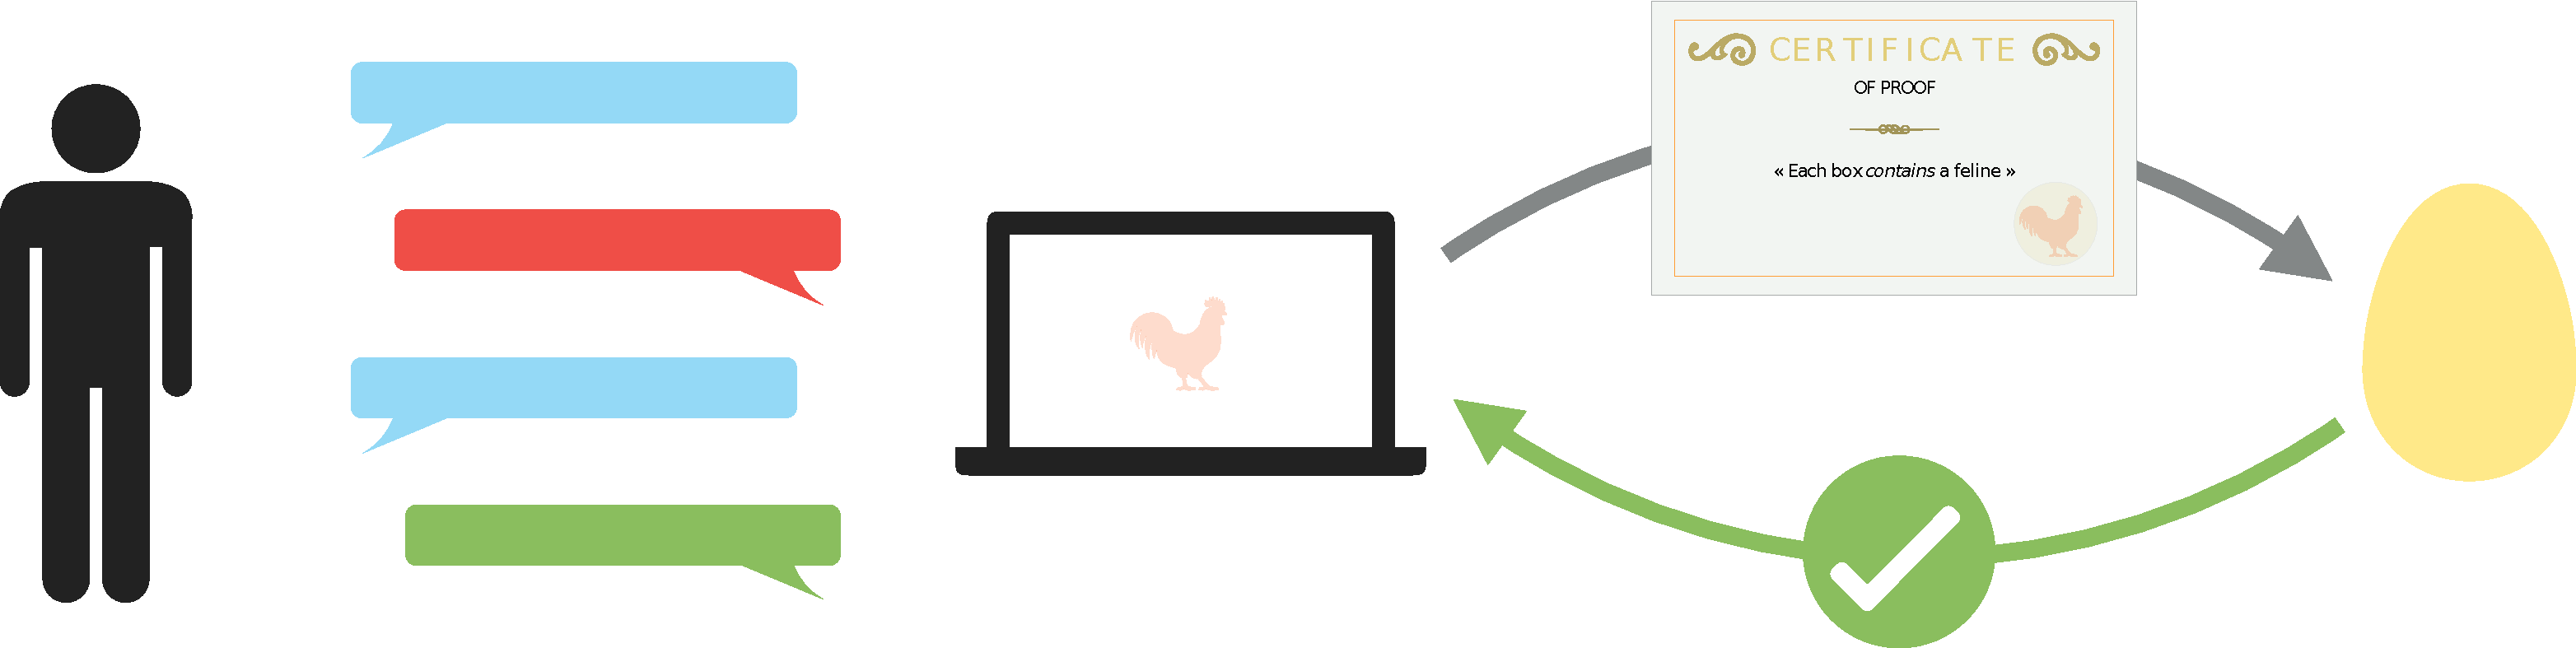
\includegraphics[width=0.9\textwidth]{chatbot-kernel.pdf}
\end{center}

If the proof assistant is broken, the certificate will be incorrect and rejected
by the kernel. As long as the kernel is correct, it is not crucial that the rest
is completly correct. Granted, it is nicer when everything is correct, but only
the correctness of the kernel is crucial.
As I said, efforts are made to keep the kernel as small as possible so that
humans can inspect it and assert of its correctness.

Unfortunately even a proof assistant as widely used as \Coq is not exempt from
mistakes: one critical bug had been found roughly every year for the past twenty
years. These are usually fixed rather fast but their mere existence is
troublesome nonetheless.
An incorrect proof can have desastrous consequences. \Coq is not only used to
prove mathematical theorems, but also to verify programs and make sure they will
not crash or end up in unwanted configurations. Such programs that we want to
verify are often used in critical parts of softwares, for instance in autopilots
and rockets, where the smallest mistake can cost millions... and lives.

I am part of a project to specificy and verify \Coq's kernel itself, within
\Coq. This means we produce a separate kernel, fully written and verified in
\Coq that can also check certificates independently.